\chapter{四足機器人}
%--------------------應用範圍反作用--------------------%
\section{應用範圍反作用}
四足機器人為一種模仿動物四肢運動方式的機器人,利用電子元件驅動機械臂可以做出許多人類難以完成的任務,同時為人們帶來許多樂趣及益處。可大致上分為以下幾項\\

1.軍事:四足機器人有良好的機械性能,搭配著電子控制系統,可以輕鬆在各地形中運輸物品及人員,透過感測器的回饋,調適馬達的行程及出力大小,在戰場中穿梭及運輸補給品,或是在搜救行動也可以當作先鋒隊,減少搜救人員的危險性並增加搜救的效率。\\

2.工業:減少作業人員在高風險環境中造成職業傷害,並保持高效的運作,減少工業中的資源浪費,在醫療機構中可以減少醫護人員的職業暴露、並經過充分消毒後也可以成為照顧病人的工具之一。\\

3.民生:四足機器人也可以當作寵物飼養,陪伴主人進行各種活動,並且可以執行各種指令,在主人發生意外時或危險發生時可以主動通報主人或救護單位,也可幫助年老或行動不便者的各種需求,也可以模組化各部件,讓人們可以依照需求進行各式改裝及編成。\\

隨著電腦的普及,各式各樣的編程軟體如雨後春筍般誕生,並且計算機語言也日益精簡,讓更多使用者可以輕而易舉的使用,網路上也有許多工程師分享開源的程式可以參考及學習。\\[6pt]
\newpage
%----------------機械手臂運動學模型---------------%
\section{步行結構運動學模型介紹}

在步行結構設計之初,設計者通常通過模仿生物腿部來創造不同的機械模型,不同型態的機械模型都有其各自特性,對於連接機構的運動控制,一般來說,腿部的機械結構不能過於複雜,過多的機械零件需要較精細的控制元件及設計、製造成本,對於控制運動軌跡來說較不益,以三連桿及四連桿閉環機構介紹。\\
\subsection{步行結構運動學模型介紹}
1.三連桿運動機構\\
為三個結構組成,以生物的身體構造解釋,可分為髖關節、大腿、小腿,結構以一個關節連接本體,對於此種機構,優點在於結構較為緊湊、簡單,通過控制三連桿關節的旋轉角度,控制尾端的位置,達到目標動作及整體姿態。\\

2.四閉環連接機構\\
為四個結構連桿組成一個不規則四邊形,有著兩個馬達分別驅動A、B桿,通過A、B桿的搖擺可以讓連桿有大幅度的運動,此機構較為複雜,需要精細的控制才能實現較穩定的運動,但有著能承受較大負載的優勢,對於運動穩定性也有著良好的表現,也是這個專題研究為何會選擇此機構的原因之一。\\
\newpage

%----------------硬體架構---------------%
\section{硬體架構}
----------------------圖片-----------------------------------------圖片-------------------
----------------------介紹-----------------------------------------介紹-------------------
----------------------圖片-----------------------------------------圖片-------------------
----------------------介紹-----------------------------------------介紹-------------------
----------------------圖片-----------------------------------------圖片-------------------
----------------------介紹-----------------------------------------介紹-------------------
----------------------圖片-----------------------------------------圖片-------------------
----------------------介紹-----------------------------------------介紹-------------------
\newpage

%-------------四連桿機構運動學模型---------------%
\section{四連桿機構運動學模型}

四連桿機構最早可以追朔到19世紀末的機械工程領域,用於織布機的機械結構,由四個桿件及四個轉動連接點組成,形成一個不規則的四邊形閉環,可以控制機械的運動軌跡及速度,實現自動化編織過程。\\
在現代,四連桿閉環機構被廣泛用於機械工業、機器人技術等領域。作為機器人的關節結構有靈活、平穩、高負載、高自由度等特性,使成為此領域重要結構之一,隨著科技的發展人們也不斷對此機構進行改進和創新、優化以滿足更多的應用需求。\\

……………………四連桿目標位置公式….………………..

\subsection{順向運動學}
順向運動學公式是用以計算末端點位置及姿態的數學公式,該公式由矩陣組成,主要利用幾何關係與向量代數以求解四連桿機構的運動學參數及目標位置、速度、角度。\
首先建立四連桿機構運動學模型,設定關節角度、連桿長度、連桿偏移量等參數,接著利用上述所提到的代數和幾何關係求解步行機構的目標位置等參數。\\

\begin{figure}[hbt!]
\begin{center}
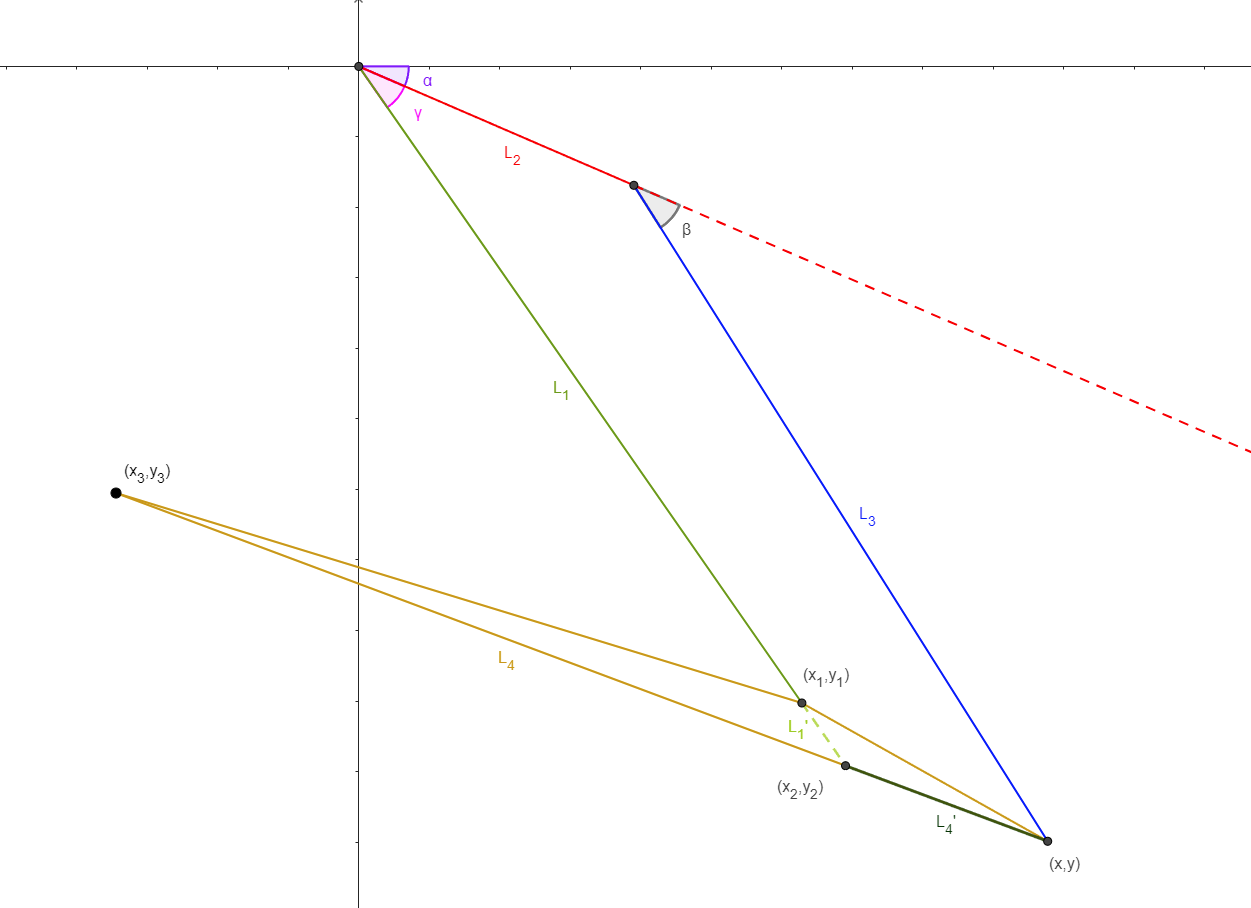
\includegraphics[angle=90,width=10cm]{Forward kinematics formula}
\caption{\Large 四連趕機構}\label{Forward kinematics formula}
\end{center}
\end{figure}

(X,Y)座標    
\[
\begin{aligned}
x=L_{1}\cos \alpha +L_{2}\cos \left( \alpha +\beta \right)\\
y=L_{1}\sin \alpha +L_{2}\sin \left( \alpha +\beta \right) 
\end{aligned}
\]

Z長度
\[
\begin{aligned}
z^{2}=\sqrt{L_{1}^{2}+L_{2}^{2}-2\times L_{1}\times L_{2}\times \cos \left( 180-\beta \right) }\\
\phi =\cos ^{-1}\dfrac{z^{2}+L_{1}^{2}-L_{2}^{2}}{2z\times L_{1}}
\end{aligned}
\]

\[
\begin{aligned}
x'=L_{4}\cos \left( \alpha +\theta \right)\\
y'=L_{4}\sin \left( \alpha +\theta \right)
\end{aligned}
\]
假設
L3:L3'=3:2
\[
\begin{aligned}
x''=\left( x'-x\right) \times \dfrac{L3}{L3'}\\
y''=\left( y'-y\right) \times \dfrac{L3}{L3'}
\end{aligned}
\]

將步行機構的參數套入此公式,給定各連桿及方向和位置,接著將各關節的象隊座標矩陣相乘,即可以推導四連桿機構的目標位置\\

---------------------------參數帶入公式-----------------------------------


由此公式可得出目標點相對於基座連結關節的座標\\

\subsection{逆向運動學}
跟順向運動學不同是,此種求解方法需要先定義目標位置和姿態,通過觀察機械系統的末端效應來推導出機械系統中各個關節的運動學問題,通常可以表示為一個非線性方程組問題,其中每個方程都可都代表著一個機械臂關節的末端位置及角度,這些方程一般都是非線性的,因此需要使用數值方法去求解。\\
逆項運動學作用於機器人在空間中精準控制末端姿態,在機器臂控制、機器人視覺和機器人運動學等領域有著許多應用的地方。\\

%-------------------硬體架構----------------%
\section{硬體架構}
 
 %-----------------軟體架構-----------------%
 \section{軟體架構}
\begin{figure}[hbt!]
\begin{center}
\includegraphics[height=8cm]{pong_gym}
\caption{\Large ATARI Pong}\label{fig.pong}
\end{center}
\end{figure} 

\newpage
